\documentclass[border=0.2in]{standalone}
\usepackage{tikz}
\usepackage{xcolor}
\usetikzlibrary{shapes.misc, patterns}

\begin{document}
%%%%%%%%%%%%%%%%%%%%%%%%%%%%%%%%%%%%%%%%%%%%%%%%%%
%%%%%%%%%%%%%%%%%%%%%%%%%%%%%%%%%%%%%%%%%%%%%%%%%%
\begin{tabular}{c c}

%%% Color fill
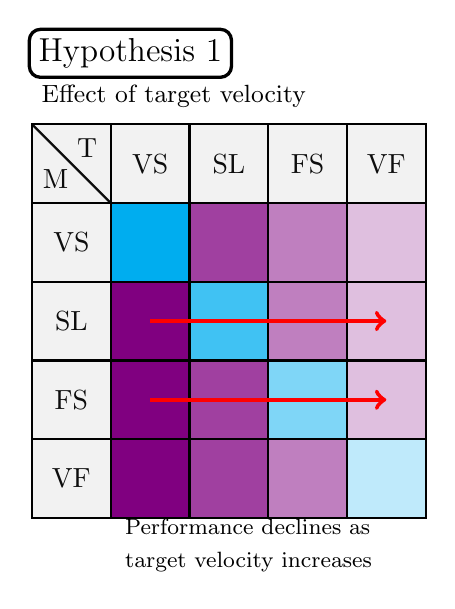
\begin{tikzpicture}
  % Prediction label
  \node[draw, very thick, rounded corners] at (1.25, 5.9) {\large Hypothesis 1};
  \node at (1.8, 5.35) {\small Effect of target velocity};

  % Target/Masker
  \node at (0.7, 4.7) {T};
  \node at (0.3, 4.3) {M};
  \draw[thick] (0, 5) -- (1, 4);
  
  % Row labels
  \node at (1.5, 4.5) {VS};
  \node at (2.5, 4.5) {SL};
  \node at (3.5, 4.5) {FS};
  \node at (4.5, 4.5) {VF};
  % Column labels
  \node at (0.5, 3.5) {VS};
  \node at (0.5, 2.5) {SL};
  \node at (0.5, 1.5) {FS};
  \node at (0.5, 0.5) {VF};
  
  % Row 1 (top)
  \draw[thick, draw=black, fill=gray, fill opacity=0.1]
     (0, 4) -- (0, 5) -- (1, 5) -- (1, 4) -- cycle;
  \draw[thick, draw=black, fill=gray, fill opacity=0.1]
     (1, 4) -- (1, 5) -- (2, 5) -- (2, 4) -- cycle;
  \draw[thick, draw=black, fill=gray, fill opacity=0.1]
     (2, 4) -- (2, 5) -- (3, 5) -- (3, 4) -- cycle;
  \draw[thick, draw=black, fill=gray, fill opacity=0.1]
     (3, 4) -- (3, 5) -- (4, 5) -- (4, 4) -- cycle;
  \draw[thick, draw=black, fill=gray, fill opacity=0.1]
     (4, 4) -- (4, 5) -- (5, 5) -- (5, 4) -- cycle;
  % Row 2
  \draw[thick, draw=black, fill=gray, fill opacity=0.1]
     (0, 3) -- (0, 4) -- (1, 4) -- (1, 3) -- cycle;
  \draw[thick, draw=black, fill=cyan, fill opacity=1.]
     (1, 3) -- (1, 4) -- (2, 4) -- (2, 3) -- cycle;
  \draw[thick, draw=black, fill=violet, fill opacity=0.75]
     (2, 3) -- (2, 4) -- (3, 4) -- (3, 3) -- cycle;
  \draw[thick, draw=black, fill=violet, fill opacity=0.5]
     (3, 3) -- (3, 4) -- (4, 4) -- (4, 3) -- cycle;
  \draw[thick, draw=black, fill=violet, fill opacity=0.25]
     (4, 3) -- (4, 4) -- (5, 4) -- (5, 3) -- cycle;
  % Row 3
  \draw[thick, draw=black, fill=gray, fill opacity=0.1]
     (0, 2) -- (0, 3) -- (1, 3) -- (1, 2) -- cycle;
  \draw[thick, draw=black, fill=violet, fill opacity=1.]
     (1, 2) -- (1, 3) -- (2, 3) -- (2, 2) -- cycle;
  \draw[thick, draw=black, fill=cyan, fill opacity=0.75]
     (2, 2) -- (2, 3) -- (3, 3) -- (3, 2) -- cycle;
  \draw[thick, draw=black, fill=violet, fill opacity=0.5]
     (3, 2) -- (3, 3) -- (4, 3) -- (4, 2) -- cycle;
  \draw[thick, draw=black, fill=violet, fill opacity=0.25]
     (4, 2) -- (4, 3) -- (5, 3) -- (5, 2) -- cycle;
  % Row 4
  \draw[thick, draw=black, fill=gray, fill opacity=0.1]
     (0, 1) -- (0, 2) -- (1, 2) -- (1, 1) -- cycle;
  \draw[thick, draw=black, fill=violet, fill opacity=1.]
     (1, 1) -- (1, 2) -- (2, 2) -- (2, 1) -- cycle;
  \draw[thick, draw=black, fill=violet, fill opacity=0.75]
     (2, 1) -- (2, 2) -- (3, 2) -- (3, 1) -- cycle;
  \draw[thick, draw=black, fill=cyan, fill opacity=0.5]
     (3, 1) -- (3, 2) -- (4, 2) -- (4, 1) -- cycle;
  \draw[thick, draw=black, fill=violet, fill opacity=0.25]
     (4, 1) -- (4, 2) -- (5, 2) -- (5, 1) -- cycle;
  % Row 5 (bottom)
  \draw[thick, draw=black, fill=gray, fill opacity=0.1]
     (0, 0) -- (0, 1) -- (1, 1) -- (1, 0) -- cycle;
  \draw[thick, draw=black, fill=violet, fill opacity=1.]
     (1, 0) -- (1, 1) -- (2, 1) -- (2, 0) -- cycle;
  \draw[thick, draw=black, fill=violet, fill opacity=0.75]
     (2, 0) -- (2, 1) -- (3, 1) -- (3, 0) -- cycle;
  \draw[thick, draw=black, fill=violet, fill opacity=0.5]
     (3, 0) -- (3, 1) -- (4, 1) -- (4, 0) -- cycle;
  \draw[thick, draw=black, fill=cyan, fill opacity=0.25]
     (4, 0) -- (4, 1) -- (5, 1) -- (5, 0) -- cycle;
  
  % Prediction help
  \draw[help lines, ->, red, ultra thick] (1.5, 2.5) -- (4.5, 2.5);
  \draw[help lines, ->, red, ultra thick] (1.5, 1.5) -- (4.5, 1.5);
  \node[align=left] at (2.75, -0.35) {\footnotesize Performance declines as\\\footnotesize target velocity increases};
\end{tikzpicture}
&



%%% Color fill
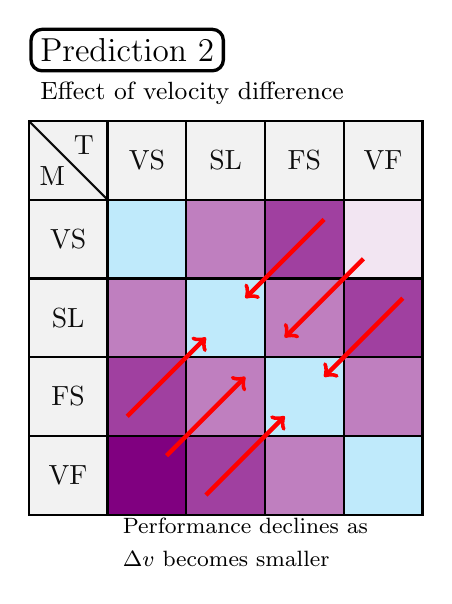
\begin{tikzpicture}
  % Prediction label
  \node[draw, very thick, rounded corners] at (1.25, 5.9) {\large Prediction 2};
  \node at (2.075, 5.35) {\small Effect of velocity difference};
  
  % Target/Masker
  \node at (0.7, 4.7) {T};
  \node at (0.3, 4.3) {M};
  \draw[thick] (0, 5) -- (1, 4);
  
  % Row labels
  \node at (1.5, 4.5) {VS};
  \node at (2.5, 4.5) {SL};
  \node at (3.5, 4.5) {FS};
  \node at (4.5, 4.5) {VF};
  % Column labels
  \node at (0.5, 3.5) {VS};
  \node at (0.5, 2.5) {SL};
  \node at (0.5, 1.5) {FS};
  \node at (0.5, 0.5) {VF};
  
  % Row 1 (top)
  \draw[thick, draw=black, fill=gray, fill opacity=0.1]
     (0, 4) -- (0, 5) -- (1, 5) -- (1, 4) -- cycle;
  \draw[thick, draw=black, fill=gray, fill opacity=0.1]
     (1, 4) -- (1, 5) -- (2, 5) -- (2, 4) -- cycle;
  \draw[thick, draw=black, fill=gray, fill opacity=0.1]
     (2, 4) -- (2, 5) -- (3, 5) -- (3, 4) -- cycle;
  \draw[thick, draw=black, fill=gray, fill opacity=0.1]
     (3, 4) -- (3, 5) -- (4, 5) -- (4, 4) -- cycle;
  \draw[thick, draw=black, fill=gray, fill opacity=0.1]
     (4, 4) -- (4, 5) -- (5, 5) -- (5, 4) -- cycle;
  % Row 2
  \draw[thick, draw=black, fill=gray, fill opacity=0.1]
     (0, 3) -- (0, 4) -- (1, 4) -- (1, 3) -- cycle;
  \draw[thick, draw=black, fill=cyan, fill opacity=0.25]
     (1, 3) -- (1, 4) -- (2, 4) -- (2, 3) -- cycle;
  \draw[thick, draw=black, fill=violet, fill opacity=0.5]
     (2, 3) -- (2, 4) -- (3, 4) -- (3, 3) -- cycle;
  \draw[thick, draw=black, fill=violet, fill opacity=0.75]
     (3, 3) -- (3, 4) -- (4, 4) -- (4, 3) -- cycle;
  \draw[thick, draw=black, fill=violet, fill opacity=0.1.]
     (4, 3) -- (4, 4) -- (5, 4) -- (5, 3) -- cycle;
  % Row 3
  \draw[thick, draw=black, fill=gray, fill opacity=0.1]
     (0, 2) -- (0, 3) -- (1, 3) -- (1, 2) -- cycle;
  \draw[thick, draw=black, fill=violet, fill opacity=0.5]
     (1, 2) -- (1, 3) -- (2, 3) -- (2, 2) -- cycle;
  \draw[thick, draw=black, fill=cyan, fill opacity=0.25]
     (2, 2) -- (2, 3) -- (3, 3) -- (3, 2) -- cycle;
  \draw[thick, draw=black, fill=violet, fill opacity=0.5]
     (3, 2) -- (3, 3) -- (4, 3) -- (4, 2) -- cycle;
  \draw[thick, draw=black, fill=violet, fill opacity=0.75]
     (4, 2) -- (4, 3) -- (5, 3) -- (5, 2) -- cycle;
  % Row 4
  \draw[thick, draw=black, fill=gray, fill opacity=0.1]
     (0, 1) -- (0, 2) -- (1, 2) -- (1, 1) -- cycle;
  \draw[thick, draw=black, fill=violet, fill opacity=0.75]
     (1, 1) -- (1, 2) -- (2, 2) -- (2, 1) -- cycle;
  \draw[thick, draw=black, fill=violet, fill opacity=0.5]
     (2, 1) -- (2, 2) -- (3, 2) -- (3, 1) -- cycle;
  \draw[thick, draw=black, fill=cyan, fill opacity=0.25]
     (3, 1) -- (3, 2) -- (4, 2) -- (4, 1) -- cycle;
  \draw[thick, draw=black, fill=violet, fill opacity=0.5]
     (4, 1) -- (4, 2) -- (5, 2) -- (5, 1) -- cycle;
  % Row 5 (bottom)
  \draw[thick, draw=black, fill=gray, fill opacity=0.1]
     (0, 0) -- (0, 1) -- (1, 1) -- (1, 0) -- cycle;
  \draw[thick, draw=black, fill=violet, fill opacity=1.]
     (1, 0) -- (1, 1) -- (2, 1) -- (2, 0) -- cycle;
  \draw[thick, draw=black, fill=violet, fill opacity=0.75]
     (2, 0) -- (2, 1) -- (3, 1) -- (3, 0) -- cycle;
  \draw[thick, draw=black, fill=violet, fill opacity=0.5]
     (3, 0) -- (3, 1) -- (4, 1) -- (4, 0) -- cycle;
  \draw[thick, draw=black, fill=cyan, fill opacity=0.25]
     (4, 0) -- (4, 1) -- (5, 1) -- (5, 0) -- cycle;
  
  % Prediction help
  \draw[help lines, ->, red, ultra thick] (1.25, 1.25) -- (2.25, 2.25);
  \draw[help lines, ->, red, ultra thick] (1.75, 0.75) -- (2.75, 1.75);
  \draw[help lines, ->, red, ultra thick] (2.25, 0.25) -- (3.25, 1.25);
  \draw[help lines, <-, red, ultra thick] (2.75, 2.75) -- (3.75, 3.75);
  \draw[help lines, <-, red, ultra thick] (3.25, 2.25) -- (4.25, 3.25);
  \draw[help lines, <-, red, ultra thick] (3.75, 1.75) -- (4.75, 2.75);
  \node[align=left] at (2.75, -0.35) {\footnotesize Performance declines as\\\footnotesize $\Delta v$ becomes smaller};
\end{tikzpicture}

\end{tabular}

%%%%%%%%%%%%%%%%%%%%%%%%%%%%%%%%%%%%%%%%%%%%%%%%%%
%%%%%%%%%%%%%%%%%%%%%%%%%%%%%%%%%%%%%%%%%%%%%%%%%%
\end{document}